\section{Sequential AIR}

Let us start describing the model from the point of view of its generative story. Images are generated by first assuming that, at every time-step, objects are propagated from previous time-step and some new objects can be introduced. Let $k \in \{0, 1, \dots, K\}$, $K \in \mathcal{N}_+$ the number of objects propagated from the previous time-step and let $n \in \{0, 1, \dots, N - k\}$, $N \in \mathcal{N}_+$ the number of objects discovered at the current time-step. Note that the maximum of $K$ objects can be propagated and the model can handle up to $N$ total objects, therefore $K \leq N$. 

Let superscripts $D$ and $P$ denote latent variables generated by discovery and propagation models, respectively. At the first time-step $t = 1$ there are no objects to propagate, so we sample up to $N$ objects from a discovery prior $\p{n_1, \bz_1^D}{N}$. Starting from the second time-step $t=2$, the model first propagates objects by sampling from a propagation prior $\p{k_2, \bz_2^P}{n_1 + k_1, \bz_1}$, where $\bz_1 = \bz_1^D$. The model also samples $n_2$ new objects from the prior $\p{n_2, \bz_2^D}{N - k_2}$. From now on, that is for $t \geq 2$, we set the aggregated latent variable $\bz_t = \{\bz_t^P, \bz_t^D\}$. This process continues up to the final time-step $T$. The images are generated by passing the generated latent variables $\bzTs$ to the generative model $\p{\bxt}{\bzt}{\theta}$ one at a time. Note that $\bzt$ is a set of up to $N$ latent variable, where each latent variable represents a separate objects. The generating model acts separately on every latent variable in the set, and the output random variable of the generating model consists of the sum of outputs of the generative model for each latent variable in the set. \Cref{fig:seq_air} shows the graphical model of the generative story. Please that the prior for the number of new objects stays the same for every time-step and it is analogous to the prior used by AIR, with the exception that the number of maximum objects can differ.

 
The sequential model works in two stages. At every timestep, it uses the original AIR, albeit with a variable maximum number of processing steps, to discover new objects. 

\begin{figure}
    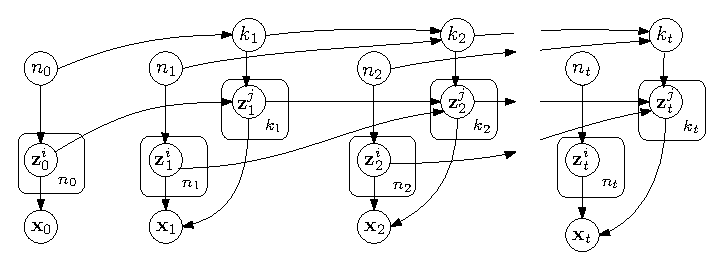
\includegraphics[width=\textwidth]{seq_air}
    \caption{The generative story of sequential AIR}
    \label{fig:seq_air}
\end{figure}

\begin{figure}
    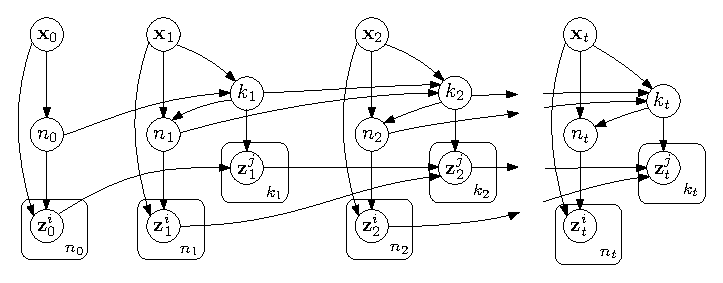
\includegraphics[width=\textwidth]{seq_air_inference}
    \caption{Graphical model for inference in sequential AIR}
    \label{fig:seq_air_inf}
\end{figure}